\chapter{Experimental configuration}



\section{The Gen IIc planar ion trap}
 
\begin{figure}[t]
    \begin{center}
        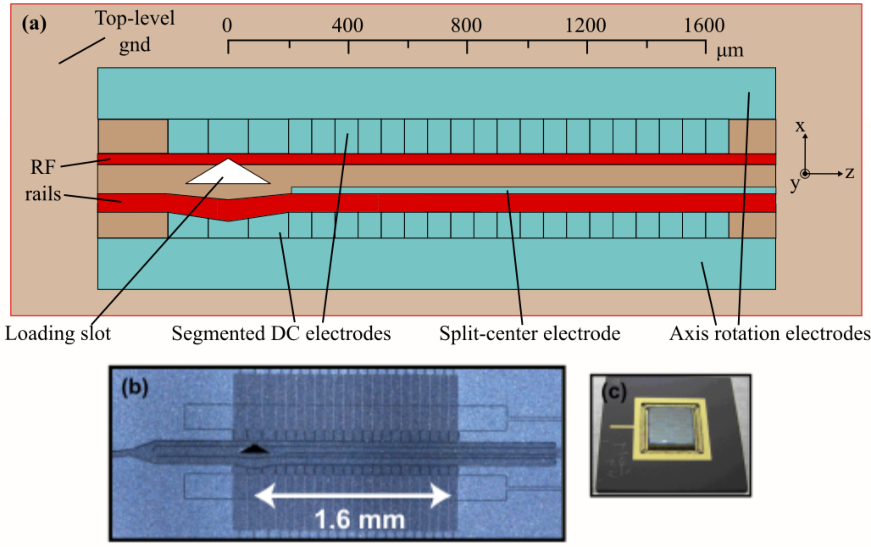
\includegraphics{figures/3/Fig_genIItrapR}
        \caption{\label{fig:genIItrap} Figures from Ref. \cite{IonTrap}. (a) Schematic view of the active trap region in the Gen IIc. (b) Optical microscope image of the active region. (c) The fabricated trap is mounted on a 100 pin CPGA for voltage control of the electrodes.   }
    \end{center}
\end{figure}

For all of the work described in this thesis we have used GTRI Gen IIc surface electrode linear ion trap (Fig. \ref{fig:genIItrap}), which transforms the linear RF trap geometry into a planar one. The design, fabrication, and performance characteristics of this trap are described in detail in Ref. \cite{IonTrap}.  The trap design is based on an asymmetric five-wire geometry \cite{FiveWire}. A pair of RF electrodes is combined with a split center DC electrode and segmented outer DC electrodes in order to provide the confining RF and DC potentials. The widths and placement of these electrodes have been chosen for a target ion height of 63 $\mu$m above the surface, and so that the radial axes are rotated approximately 20$^o$ relative to surface normal. The rotated axes allow for both radial secular modes to be Doppler cooled by a single laser parallel to the trap surface. Said modes have non-degenerate frequencies $\omega_{r1}, \ \omega_{r2} \approx (2 \pi) \times 4-6$ MHz, consistent with the values $q_i \approx 0.15$ and $a_i \approx 0.01$ which parameterize the trap. The exact frequencies vary based on factors such as stray field gradients and (as will be relevant in Ch. 4) the ion's position relative to the RF null. The single axial secular mode has a frequency $\omega_{z} \approx (2 \pi) \times 1$ MHz.

The DC segmented electrodes allow for axial transport of ions along the 1600 $\mu$m length of the active trapping region (Fig. \ref{fig:genIItrap} (a)). This is done with computer modeled sets of applied potentials on the electrodes which produce axial harmonic wells at regularly spaced intervals of around $\mu$m throughout the active region. These are referred to as the trap waveforms. Interpolation between adjacent waveforms provides harmonic wells at any position in the active region. Ion transport occurs by sequentially updating the electrodes in order to produce a moving harmonic well. Multiple wells can be generated to simultaneously trap multiple ions, as well as to merge/separate them into/from a linear chain in a single harmonic potential. Chains of 10 ions have previously been demonstrated in our trap \cite{IonTrap}. In addition, the waveforms can generate static offset fields from the electrodes which shift the ions' radial position by up to 10 $\mu$m. This used primarily for the compensation of stray electric fields which push the ion away from the RF null and increase micromotion, but can also be utilized for experimental purposes as we will see in Ch. 4.

Ion capture occurs at the location of the backside loading slot, defined as position z = 0 $\mu$m on the trap axis. A flux of neutral atoms is ejected from a coil-heated sample of material and passes through the slot. The neutral atoms are then ionized using a resonance enhanced two-photon scheme \cite{Gulde2001}, in which a resonant 423 nm laser interaction is followed by a 377 nm laser interaction, with the two lasers overlapping at the loading position. Harmonic well depths of several eV are suitable for capturing ions from the flux. 

\begin{figure}[t]
    \begin{center}
        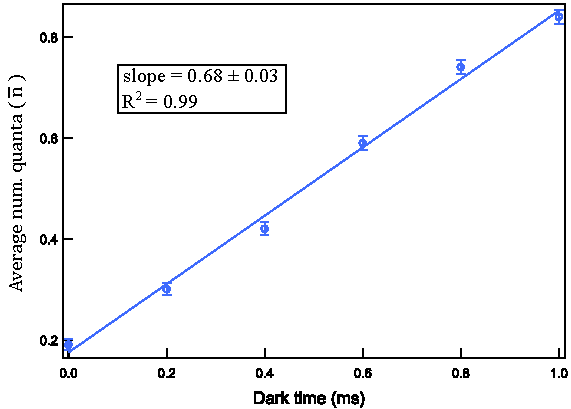
\includegraphics{figures/3/Fig_HeatingRate}
        \caption{\label{fig:heatingrate} Heating rate data for our trap: $\bar{n}$ vs. ``dark time'' (during which the ion is not actively cooled). The fitted slope gives the heating rate for our trap as $\dot{\bar{n}} \approx 680$ quanta/sec. The heating rate was measured on the 1.3 MHz axial mode. }
    \end{center}
\end{figure}


As mentioned in Sec. 2.5, heating of ions will occur due to electric field noise, fluctuating patch potentials of electrodes, etc. All traps have an inherent heating rate $\dot{\bar{n}}$ which is approximately linear in time near the ground state. By measuring $\bar{n}$ as a function of time without active cooling (``dark time''), we can determine the heating rate. In our trap we measure $\dot{\bar{n}} \approx$ 680 quanta/s on the 1.3 MHz axial mode (see Fig. \ref{fig:heatingrate}). For comparison, heating rates in similar traps are typically in the $10^2 - 10^3$ quanta/s range \cite{doi:10.1063/1.4917385, PhysRevLett.96.253003, PhysRevA.76.033411, Shu14.PRA.89.062308}.

%%%%%%%%%%%%%%%%%%%%%%%%%%%%%%
\section{Trap enclosures and fluoresence detection}

\begin{figure}[t]
    \begin{center}
        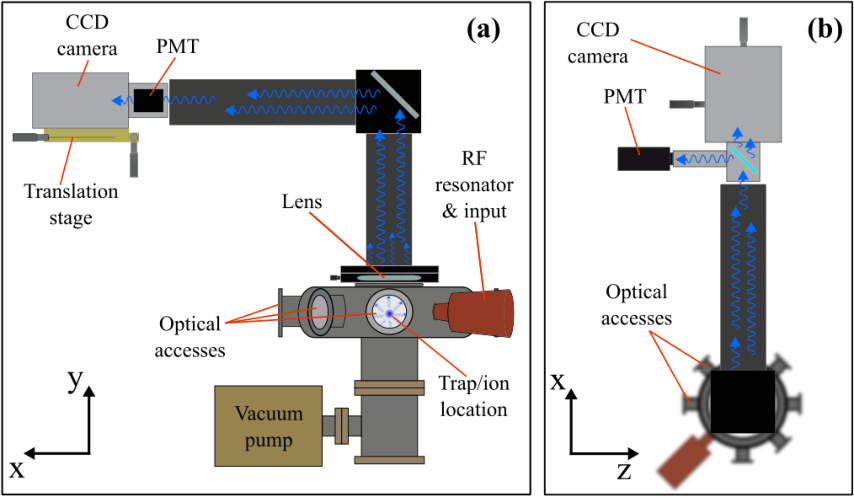
\includegraphics{figures/3/Fig_CameraConfigR}
        \caption{\label{fig:CameraConfig} Illustrated schematic of the trap's vacuum enclosure and fluoresence detection optics, in a (a) side-on and (b) top-down perspective. Description in text.   }
    \end{center}
\end{figure}


Fig. \ref{fig:CameraConfig} shows an illustrated schematic of the trap enclosure and fluorescence detection optics. The fabricated Gen IIc trap is mounted on a CPGA chip (Fig. \ref{fig:genIItrap} (c)) and enclosed in stainless steel vacuum chamber held at $\sim 10^{-12}$ torr. The circular chamber has 7 optical access windows positioned at $45^{\circ}$ intervals about its center (more detail can be seen in Fig. \ref{fig:LaserConfig}). A large top-view window allows the trap surface to be continuously imaged by a CCD camera. The optical pathway of this camera is optimized to provide a $\sim 500 \times 500$ $\mu$m$^2$ viewing area when filtered to collect 397 nm light. Ion fluorescence at 397 nm occurs any time the ion interacts with the 397 nm laser. For high speed and high fidelity state detection, a portion of this light is directed onto a photomultiplier tube (PMT) which returns photon-count measurements back to the experiment control software. The camera and PMT are mounted together on a translation stage, allowing the entire length of the trap to be imaged. 

The entire configuration is enclosed in a magnetic shielding box with a removable front lid for access. Magnetometer measurements near the trap chamber record a factor of $\sim$ 5 reduction in ambient magnetic field noise when the lid is on and the trap chamber is fully shielded. All of the experiments in this thesis were run with full shielding. 



%%%%%%%%%%%%%%%%%%%%%%%%%%%%%%
%\section{Fluorescence detection}





%%%%%%%%%%%%%%%%%%%%%%%%%%%%%%
\section{Laser hardware and trap-side configuration}

\begin{figure}[ht]
    \begin{center}
        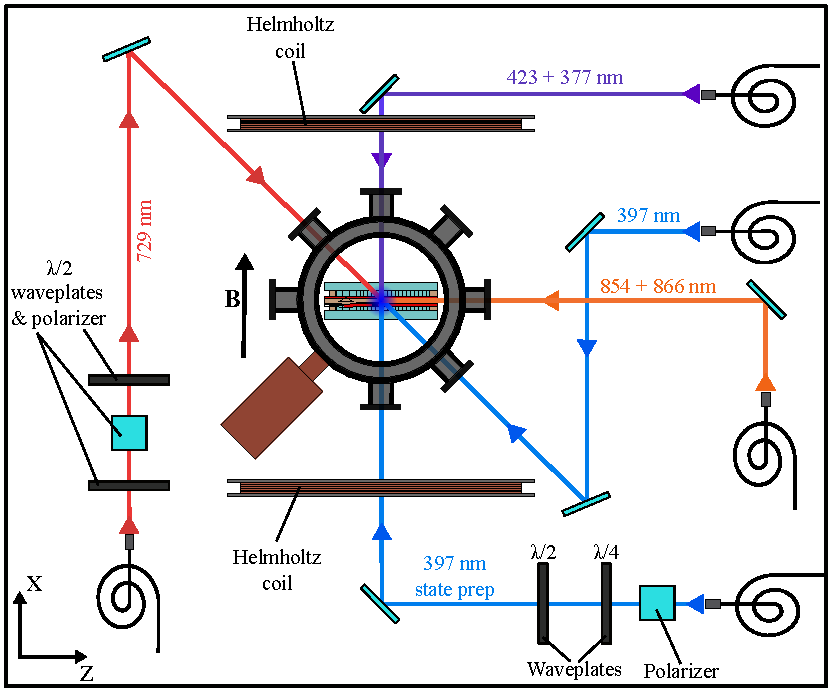
\includegraphics{figures/3/Fig_lasers5}
        \caption{\label{fig:LaserConfig} Illustrated schematic of the laser and magnetic field generation configuration at the trap chamber (trap not to scale). Fiber optic cables (black coils) bring appropriately conditioned light to the trap. A pair of Helmholtz coils produces a 4.3 G magnetic field in the $x$ direction. The 729 nm beam and 397 nm Doppler cooling beam are brought in at a 45$^{\circ}$ angle to the trap axis in order access/cool all secular modes. The 397 nm state preparation beam is coaxial with the $\mathbf{B}$ field. Beams pass through appropriate polarization optics when necessary. }
    \end{center}
\end{figure}

All of the laser wavelengths used in these experiments were generated with commercially available solid-state diodes and peripheral hardware. The 397, 423, 854, and 866 nm lasers are frequency stabilized to a rubidium reference source via a low finesse ($F \sim 150-200$) transfer cavity \cite{doi:10.1063/1.2337094}. The 729 nm laser is frequency stabilized in an ultra-low expansion (ULE) glass cavity via the Pound-Drever-Hall method \cite{doi:10.1119/1.1286663}. At the time of the experiments discussed in Ch. 4, the ULE cavity being used had a finesse $F \sim 10,000$ and stabilized the 729 nm linewidth to approximately 1-2 kHz. Since then it has been replaced by an $F \sim 150,000$ ULE cavity which is capable of stable linewidths in the range of 10-100 Hz.  

Frequency control of the 423 and 866 nm lasers is achieved by adjusting their stabilization set point in the transfer cavity. These beams are generally set before experiments and otherwise left static. For the 397, 729, and 854 nm beams we require dynamic control over the frequency during experiments, as well as rapid on-off switching. Both of these needs are met with Brimrose brand acousto-optical modulators (AOMs) which diffract and frequency-shift the beams with oscillating crystals. By changing the RF frequencies which drive the crystals we subsequently shift the diffracted laser frequencies, and by switching the RF drive signal on or off entirely with TTL electronics we obtain on-off control of our diffracted beams as well. The AOMs have -3 dB bandwidths typically in the 100 MHz range, and offer fast ramp-up and ramp-down times of $\sim$ 10 ns for beam switching purposes. The RF driving fields for the 397 and 729 nm beams are sourced from digital signal generators (more on these in the next section), and are amplified, TTL-switched, and otherwise modulated when necessary by Minicircuits components, primarily. 
The 397 nm beams--one for Doppler cooling and state detection, and a second for state preparation--and the 729 nm beam are in the double-pass configuration through their respective AOMs. The 854 nm beam is single-passed.

All of the appropriately conditioned light is brought to the trap chamber region via fiber-optic cables. Fig. \ref{fig:LaserConfig} shows the laser configuration entering the trap chamber. The 397 nm Doppler cooling and state detection light light is brought in at a 45$^{\circ}$ angle to the trap axis in order cool all secular modes. The state preparation 397 nm beam passes through a polarizer, a $\lambda/2$ waveplate, and $\lambda/4$ waveplate for circular polarization. The 729 nm beam passes through two $\lambda/2$ waveplates and a polarizer for optimal linear polarization, and is also incident at 45$^{\circ}$ to access all secular modes. Repump light at 854 and 866 nm is coaxial to the trap axis, and the 377 and 423 nm ionization beams are positioned at the loading slot. 

A pair of Helmholtz coils driven by a stable current source produce the 4.3 G magnetic field at the trap location. The current source is stable to within 10 $\mu$A.   


%%%%%%%%%%%%%%%%%%%%%%%%%%%%%%
\section{Signal generation, voltage control, and control software}

The RF signals which drive the AOMs for the 397 nm cooling and 729 nm beams are generated by Analog Devices AD9910 direct digital synthesizer (DDS) cards, which synchronized to a 1 GHz analog signal. These are controlled by a Xilinx XC6SLX45T-2 field programmable gate array (FPGA) device which has a 500$+$ MHz clock speed. The FPGA also controls the analog TTL signals for AOM switching, and accepts serial input signals from the PMT which correspond to photons detected. The RF signals for the 397 nm state preparation and 854 nm AOMs do not need to be updated quickly, and are therefore sourced from simple USB based devices.

DC voltages on the trap electrodes are controlled via National Instruments digital-to-analog converters which can be updated at rates of 10 kHz. They are low-pass filtered to reduce higher frequency noise. The electrode voltages reach the trap chip via access pins built into the vacuum chamber. The trap's RF drive frequency is sourced from a Hewlett-Packard analog signal generator and is amplified via a Minicircuits amplifier. The RF signal enters the trap chamber through a helical resonator, which maximizes the drive voltage on the trap surface while reducing noise \cite{Siverns2012}. Our trapping frequency $\Omega_{RF} = 52.525$ MHz is set to the resonance of the resonator. 

We use the Wavemetrics Igor software environment to control relevant hardware, run experimental procedures, and collect data. Experiments are triggered by a 60 Hz pulse sourced from the power mains in order to avoid sampling the AC magnetic field fluctuations. 

